\documentclass[9pt]{beamer}
\usetheme{Warsaw}
\usefonttheme[onlymath]{serif}

\usepackage[utf8]{inputenc}
\usepackage[polish]{babel}
\usepackage[T1]{fontenc}
\usepackage{comment}
\usepackage{setspace}
\usepackage{amsmath}
\usepackage{dcolumn}
\usepackage{siunitx}
\usepackage{tabularx}
\usepackage{graphicx}
\graphicspath{{../images/}}

\sisetup{
    table-number-alignment = center, % Align numbers at the decimal point
    table-format = 1.3e2,           % Specify number format: 1 digit before, 3 after decimal, and 1 exponent
    tight-spacing = true,           % Remove extra spacing around numbers
}

\newcolumntype{M}{>{\centering\arraybackslash\math}p{2cm}}

\newcommand{\n}{\newline}

\linespread{1}

\title{Projekt 1, Zadanie 23}
\author{Wiktor Murawski, 333255, grupa 3, środa 12:15}
\date{}


\begin{document}

\begin{frame}
    %\frametitle{\insertauthor,\space\inserttitle}

    \begin{spacing}{2}
    \begin{center}
        \inserttitle\par
        \insertauthor
    \end{center}
    \vspace{2em}
    Obliczanie całek $ \iint\limits_D f(x,y) \, dxdy $ na obszarze
    $  D = \{(x,y) \in \mathbb{R}^2 : |x| + |y| \leq 1\} $
    poprzez podział obszaru $ D $ na $ 4n^2 $ trójkątów przystających oraz
    zastosowanie na każdym z nich kwadratury rzędu drugiego.
    \end{spacing}
\end{frame}


\begin{frame}
\frametitle{Podział obszaru $D$ na $4n^2$ trójkątów przystających}
    \begin{columns}
        \column{0.5\textwidth}
        \centering
        Podział $D$ dla $n = 1$\\
        \vspace{1em}
        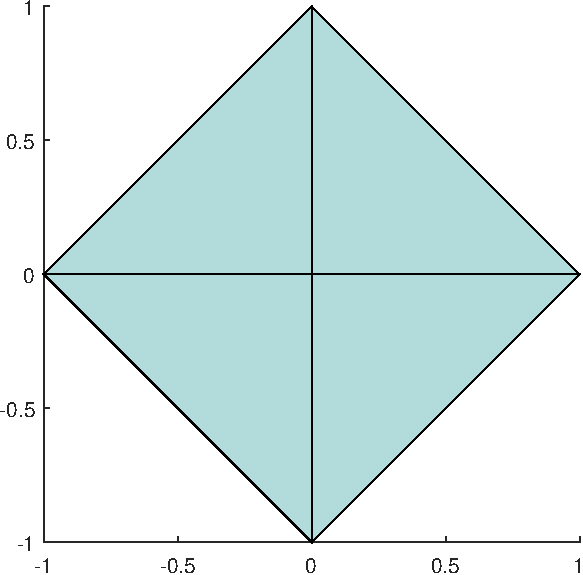
\includegraphics[width=\textwidth]{figure1.pdf}


        \column{0.5\textwidth}
        \centering
        Podział $D$ dla $n = 4$\\
        \vspace{1em}
        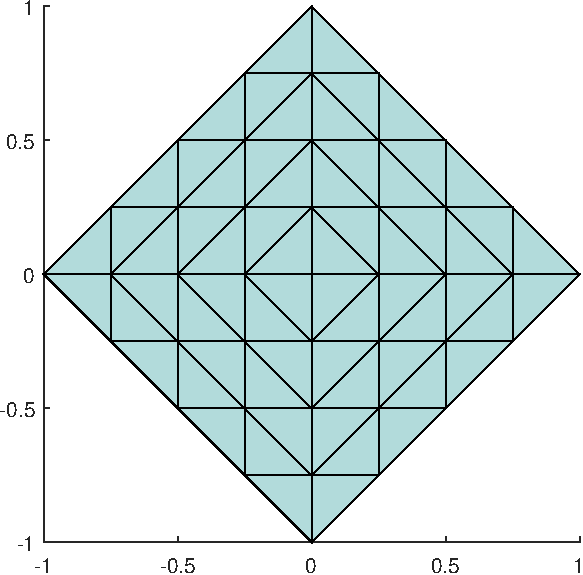
\includegraphics[width=\textwidth]{figure4.pdf}

    \end{columns}
\end{frame}


\begin{frame}
    TU MA BYĆ ALGORYTM
\end{frame}


\begin{frame}
    TU MA BYĆ OPIS KWADRATURY
\end{frame}


\begin{frame}
\frametitle{Sprawdzanie poprawności}

    \begin{spacing}{2}
        W celu sprawdzenia poprawności metody przetestujemy ją na wielomianach stopnia pierwszego.
        Obliczymy analitycznie $ I = \iint\limits_D f(x,y) \, dx dy $ gdzie
        $ f(x,y) = ax + by + c \qquad a,b,c \in \mathbb{R}$ \n
        Niech $ D_1 = \{(x,y) \in D : x \leq 0\} $ oraz $ D_2 = \{(x,y) \in D : x > 0\} $ \n
        Oznaczmy $ I_1 = \iint\limits_{D_1} f(x,y) \, dx dy $, $ I_2 = \iint\limits_{D_2} f(x,y) \, dx dy $ \n
        Wtedy $ D = D_1 \cup D_2 $ oraz $ I = I_1 + I_2 $ \n
        $ I_1 = \int\limits_{-1}^{0}\int\limits_{-x-1}^{x+1} ax+by+c \, dy dx $ \qquad\n
        $ I_2 = \int\limits_{0}^{1}\int\limits_{x-1}^{-x+1} ax+by+c \, dy dx $ \n
    \end{spacing}

\end{frame}


\begin{frame}
\frametitle{Wyznaczenie analityczne całki z funkcji stopnia 1}
    \begin{columns}
        \begin{column}{0.5\textwidth}
            % Lewa kolumna
            \begin{align*}
                I_1 &= \int\limits_{-1}^{0}\int\limits_{-x-1}^{x+1} ax+by+c \,dydx \\
                I_1 &= \int\limits_{-1}^{0}\left[axy + \frac{by^2}{2} + cy\right]_{-x-1}^{x+1} \,dx \\
                I_1 &= \int\limits_{-1}^{0} 2ax^2 + 2ax + 2cx + 2c \,dx \\
                I_1 &= 2\left[ \frac{ax^3}{3} + \frac{ax^2}{2} + \frac{cx^2}{2} + cx \right]_{-1}^{0} \\
                I_1 &= -\frac{a}{3} + c \\
            \end{align*}
        \end{column}
        \begin{column}{0.5\textwidth}
            % Prawa kolumna
            \begin{align*}
                I_2 &= \int\limits_{0}^{1}\int\limits_{x-1}^{-x+1} ax+by+c \,dydx \\
                I_2 &= \int\limits_{0}^{1}\left[axy + \frac{by^2}{2} + cy\right]_{x-1}^{-x+1} \,dx \\
                I_2 &= \int\limits_{0}^{1} - 2ax^2 + 2ax - 2cx + 2c \,dx \\
                I_2 &= 2\left[ -\frac{ax^3}{3} + \frac{ax^2}{2} - \frac{cx^2}{2} + cx \right]_{0}^{1} \\
                I_2 &= \frac{a}{3} + c \\
            \end{align*}
        \end{column}
    \end{columns}

    \begin{center}
        Ostatecznie otrzymujemy $ I = I_1 + I_2 = 2c $
    \end{center}
\end{frame}

\begin{comment}
\begin{frame}
    %\begin{table}[]
        \makebox[\textwidth]{
            \begin{tabularx}{11.22cm}{|l|l|l|l|l|l|}
                \hline
                Funkcja & Wartość z integral2 & n & Wartość & Błąd & Błąd\\
                podcałkowa & integral2 &  & obliczona & bezwzględny & względny\\
                \hline
            \end{tabularx}
        }
        \makebox[\textwidth]{
            \begin{tabularx}{\textwidth}{
                    |l
                    |S
                    |l
                    |S
                    |S
                    |S|}
                \hline
                Text1 & 1.234e+56 & 123 & 5.678e+12 & 9.876e+34 & 1.234e+56 \\
                Text2 & 9.876e+45 & 456 & 7.123e+23 & 4.567e+67 & 8.901e+45 \\
                Text3 & 2.345e+67 & 789 & 1.234e+89 & 3.456e+12 & 6.789e+67 \\
                \hline
            \end{tabularx}
        }
    %\end{table}
\end{frame}

\begin{frame}
    \begin{table}[]
        \caption{Tabela}
        \label{tab:tabela}
        \makebox[\textwidth]{
            \begin{tabular}{|l|l|l|l|l|l|}
                \hline
                Funkcja & Wartość z integral2 & n & Wartość & Błąd & Błąd\\
                podcałkowa & integral2 &  & obliczona & bezwzględny & względny\\
                \hline
            \end{tabular}
        }
    \end{table}
\end{frame}
\end{comment}



\begin{frame}

    \begin{table}[]
        %\caption{Tabela}
        %\label{tab:tabela}
        \makebox[\linewidth]{
            \begin{tabular}{|l|S|l|S|S|S|}

                \hline
                funkcja           & {wynik}      & {n}     & {wynik}     & {błąd}        & {błąd}    \\
                podcałkowa            & {dokładny}   & {}      & {uzyskany}  & {bezwzględny} & {względny}  \\
                \hline
                $f(x,y) = $   & 2.000e00 & 1   & 2.000e+00 & 1.000e-20 & 0.000e+00 \\
                $ = 1$ &          & 5   & 2.000e+00 & 1.332e-15 & 6.661e-16 \\
                &          & 10  & 2.000e+00 & 2.065e-14 & 1.033e-14 \\
                &          & 50  & 2.000e+00 & 1.876e-13 & 9.381e-14 \\
                &          & 100 & 2.000e+00 & 2.008e-12 & 1.004e-12 \\
                &          & 500 & 2.000e+00 & 1.584e-11 & 7.918e-12 \\
                \hline
                %---------------------------------------------------------------------------
                $f(x,y) = $ & 2.000e+00  & 1     & 2.000e+00   & 0.000e+00   & 0.000e+00 \\
                $ = x+y+0.5$&   & 5     & 2.000e+00   & 8.882e-16   & 4.441e-16 \\
                &   & 10    & 2.000e+00   & 2.442e-15   & 1.221e-15 \\
                &   & 50    & 2.000e+00   & 4.663e-15   & 2.331e-15 \\
                &   & 100   & 2.000e+00   & 4.885e-15   & 2.442e-15 \\
                &   & 500   & 2.000e+00   & 7.594e-14   & 3.797e-14 \\
                \hline
                %---------------------------------------------------------------------------
                $f(x,y) =$  & 6.000e+00  & 1     & 6.000e+00   & 8.882e-16   & 1.480e-16 \\
                $ = x+2y+3$ &   & 5     & 6.000e+00   & 0.000e+00   & 0.000e+00 \\
                &   & 10    & 6.000e+00   & 8.882e-16   & 1.480e-16 \\
                &   & 50    & 6.000e+00   & 8.882e-16   & 1.480e-16 \\
                &   & 100   & 6.000e+00   & 1.776e-15   & 2.961e-16 \\
                &   & 500   & 6.000e+00   & 2.665e-14   & 4.441e-15 \\
                %---------------------------------------------------------------------------
                %x+y+sqrt(2)        & 2.828e+00  & 1     & 2.828e+00   & 0.000e+00   & 0.000e+00 \\
                %        & 2.828e+00  & 5     & 2.828e+00   & 8.882e-16   & 3.140e-16 \\
                %        & 2.828e+00  & 10    & 2.828e+00   & 2.220e-15   & 7.850e-16 \\
                %        & 2.828e+00  & 50    & 2.828e+00   & 5.329e-15   & 1.884e-15 \\
                %        & 2.828e+00  & 100   & 2.828e+00   & 3.064e-14   & 1.083e-14 \\
                %        & 2.828e+00  & 500   & 2.828e+00   & 1.554e-14   & 5.495e-15 \\
                %---------------------------------------------------------------------------
                %x+y+eps & 4.441e-16  & 1     & 4.996e-16   & 5.551e-17   & 1.250e-01 \\
                %x+y+eps & 4.441e-16  & 5     & 4.441e-16   & 0.000e+00   & 0.000e+00 \\
                %x+y+eps & 4.441e-16  & 10    & 4.458e-16   & 1.735e-18   & 3.906e-03 \\
                %x+y+eps & 4.441e-16  & 50    & 4.460e-16   & 1.952e-18   & 4.395e-03 \\
                %x+y+eps & 4.441e-16  & 100   & 4.462e-16   & 2.107e-18   & 4.745e-03 \\
                %x+y+eps & 4.441e-16  & 500   & 4.426e-16   & 1.454e-18   & 3.275e-03 \\
                \hline

            \end{tabular}

        }
    \end{table}

\end{frame}

\begin{frame}
    TESTY NUMERYCZNE
\end{frame}


\begin{frame}
    TU MA BYĆ WYKRES
\end{frame}


\end{document}